%% This is the ctufit-thesis example file. It is used to produce theses
%% for submission to Czech Technical University, Faculty of Information Technology.
%%
%% Get the newest version from
%% https://gitlab.fit.cvut.cz/theses-templates/FITthesis-LaTeX
%%
%%
%% Copyright 2021, Eliska Sestakova and Ondrej Guth
%%
%% This work may be distributed and/or modified under the
%% conditions of the LaTeX Project Public Licenese, either version 1.3
%% of this license or (at your option) any later version.
%% The latest version of this license is in
%%  https://www.latex-project.org/lppl.txt
%% and version 1.3 or later is part of all distributions of LaTeX
%% version 2005/12/01 or later.
%%
%% This work has the LPPL maintenance status `maintained'.
%%
%% The current maintainer of this work is Ondrej Guth.
%% Contact ondrej.guth@fit.cvut.cz for bug reports.
%% Alternatively, submit bug reports into the tracker at
%% https://gitlab.fit.cvut.cz/theses-templates/FITthesis-LaTeX/issues
%%
%%

%%%%%%%%%%%%%%%%%%%%%%%%%%%%%%%%%%%%%%%%%
% CLASS OPTIONS
% language: czech/english/slovak
% thesis type: bachelor/master/dissertation
%%%%%%%%%%%%%%%%%%%%%%%%%%%%%%%%%%%%%%%%%
\documentclass[english,master,unicode]{ctufit-thesis}

%%%%%%%%%%%%%%%%%%%%%%%%%%%%%%%%%%
% FILL IN THIS INFORMATION
%%%%%%%%%%%%%%%%%%%%%%%%%%%%%%%%%%
\ctufittitle{Math expression evaluator for literal types in TypeScript} % replace with the title of your thesis
\ctufitauthorfull{Bc. Tat Dat Duong} % replace with your full name (first name(s) and then family name(s) / surname(s)) including academic degrees
\ctufitauthorsurnames{Duong} % replace with your surname(s) / family name(s)
\ctufitauthorgivennames{Tat Dat} % replace with your first name(s) / given name(s)
\ctufitsupervisor{Ing.\,Jaroslav Šmolík} % replace with name of your supervisor/advisor (include academic degrees)
\ctufitdepartment{Department of Software Engineering} % replace with the department of your defence
\ctufityear{2023} % replace with the year of your defence
\ctufitdeclarationplace{Prague} % replace with the place where you sign the declaration
\ctufitdeclarationdate{\today} % replace with the date of signature of the declaration
\ctufitabstractCZE{Fill in abstract of this thesis in Czech language. Class aptent taciti sociosqu ad litora torquent per conubia nostra, per inceptos hymenaeos. Cras pede libero, dapibus nec, pretium sit amet, tempor quis. Sed vel lectus. Donec odio tempus molestie, porttitor ut, iaculis quis, sem. Suspendisse sagittis ultrices augue.}
\ctufitabstractENG{Fill in abstract of this thesis in English language. Class aptent taciti sociosqu ad litora torquent per conubia nostra, per inceptos hymenaeos. Cras pede libero, dapibus nec, pretium sit amet, tempor quis. Sed vel lectus. Donec odio tempus molestie, porttitor ut, iaculis quis, sem. Suspendisse sagittis ultrices augue.}
\ctufitkeywordsCZE{enter, commma, separated, list, of, keywords, in, CZECH}
\ctufitkeywordsENG{enter, commma, separated, list, of, keywords, in, ENGLISH}
%%%%%%%%%%%%%%%%%%%%%%%%%%%%%%%%%%
% END FILL IN
%%%%%%%%%%%%%%%%%%%%%%%%%%%%%%%%%%

%%%%%%%%%%%%%%%%%%%%%%%%%%%%%%%%%%
% CUSTOMIZATION of this template
% Skip this part or alter it if you know what you are doing.
%%%%%%%%%%%%%%%%%%%%%%%%%%%%%%%%%%

\RequirePackage{iftex}[2020/03/06]
\iftutex % XeLaTeX and LuaLaTeX
    \RequirePackage{ellipsis}[2020/05/22] %ellipsis workaround for XeLaTeX
\else
    \RequirePackage[utf8]{inputenc}[2018/08/11] %this file encoding
    \RequirePackage{lmodern}[2009/10/30] % vector flavor of Computer Modern font
\fi

% hyperlinks
\RequirePackage[pdfpagelayout=TwoPageRight,colorlinks=false,allcolors=decoration,pdfborder={0 0 0.1}]{hyperref}[2020-05-15]

% uncomment the following to hide all hyperlinks
% \RequirePackage[pdfpagelayout=TwoPageRight,hidelinks]{hyperref}[2020-05-15]

\RequirePackage{pdfpages}[2020/01/28]

\setcounter{secnumdepth}{4} % numbering sections; 4: subsubsection



%%%%%%%%%%%%%%%%%%%%%%%%%%%%%%%%%%
% CUSTOMIZATION of this template END
%%%%%%%%%%%%%%%%%%%%%%%%%%%%%%%%%%


%%%%%%%%%%%%%%%%%%%%%%
% DEMO CONTENTS SETTINGS
% You may choose to modify this part.
%%%%%%%%%%%%%%%%%%%%%%
\usepackage{dirtree}
\usepackage{lipsum,tikz}
\usepackage{csquotes}
\usepackage[style=iso-numeric]{biblatex}
\addbibresource{sources.bib}
\usepackage{listings} % typesetting of sources
% \usepackage{minted} % typesetting of sources

%theorems, definitions, etc.
\theoremstyle{plain}
\newtheorem{theorem}{Věta}
\newtheorem{lemma}[theorem]{Tvrzení}
\newtheorem{corollary}[theorem]{Důsledek}
\newtheorem{proposition}[theorem]{Návrh}
\newtheorem{definition}[theorem]{Definice}
\theoremstyle{definition}
\newtheorem{example}[theorem]{Příklad}
\theoremstyle{remark}
\newtheorem{note}[theorem]{Poznámka}
\newtheorem*{note*}{Poznámka}
\newtheorem{remark}[theorem]{Pozorování}
\newtheorem*{remark*}{Pozorování}
\numberwithin{theorem}{chapter}
%theorems, definitions, etc. END
%%%%%%%%%%%%%%%%%%%%%%
% DEMO CONTENTS SETTINGS END
%%%%%%%%%%%%%%%%%%%%%%

\onehalfspacing
\NewDocumentCommand{\codeword}{v}{%
  \texttt{\textcolor{blue}{#1}}%
}

\begin{document} 
\frontmatter\frontmatterinit % do not remove these two commands

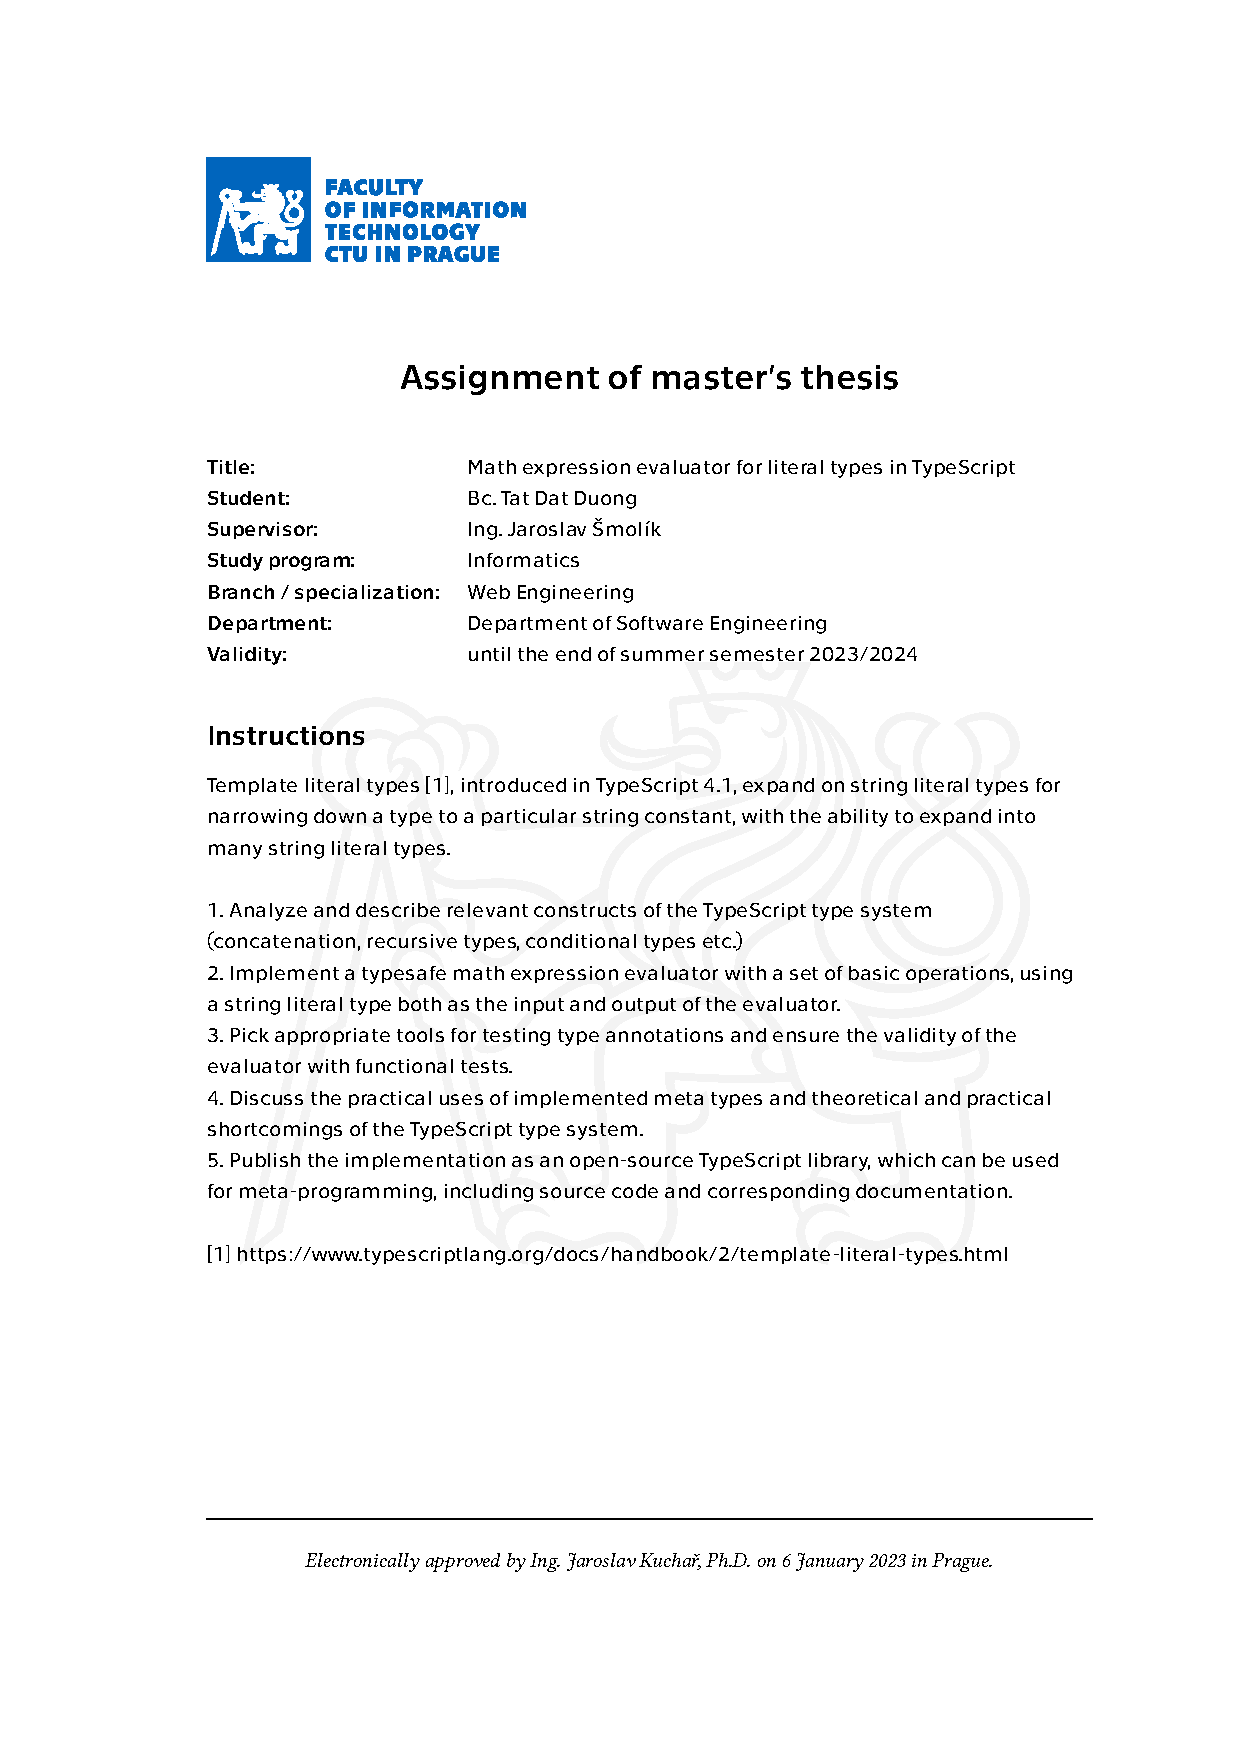
\includepdf{assignment-include.pdf} % replace that file with your thesis assignment provided by study office

\thispagestyle{empty}\cleardoublepage\maketitle % do not remove these three commands

\imprintpage % do not remove this command

\tableofcontents % do not remove this command
%%%%%%%%%%%%%%%%%%%%%%
% list of other contents: figures, tables, code listings, algorithms, etc.
% add/remove commands accordingly
%%%%%%%%%%%%%%%%%%%%%%
\listoffigures % list of figures
\begingroup
\let\clearpage\relax
\listoftables % list of tables
\lstlistoflistings % list of source code listings generated by the listings package
% \listoflistings % list of source code listings generated by the minted package
\endgroup
%%%%%%%%%%%%%%%%%%%%%%
% list of other contents END
%%%%%%%%%%%%%%%%%%%%%%

%%%%%%%%%%%%%%%%%%%
% ACKNOWLEDGMENT
% FILL IN / MODIFY
% This is a place to thank people for helping you. It is common to thank your supervisor.
%%%%%%%%%%%%%%%%%%%
\begin{acknowledgmentpage}
	Chtěl bych poděkovat především sit amet, consectetuer adipiscing elit. Curabitur sagittis hendrerit ante. Class aptent taciti sociosqu ad litora torquent per conubia nostra, per inceptos hymenaeos. Cras pede libero, dapibus nec, pretium sit amet, tempor quis. Sed vel lectus. Donec odio tempus molestie, porttitor ut, iaculis quis, sem. Suspendisse sagittis ultrices augue.
\end{acknowledgmentpage} 
%%%%%%%%%%%%%%%%%%%
% ACKNOWLEDGMENT END
%%%%%%%%%%%%%%%%%%%


%%%%%%%%%%%%%%%%%%%
% DECLARATION
% FILL IN / MODIFY
%%%%%%%%%%%%%%%%%%%
% INSTRUCTIONS
% ENG: choose one of approved texts of the declaration. DO NOT CREATE YOUR OWN. Find the approved texts at https://courses.fit.cvut.cz/SFE/download/index.html#_documents (document Declaration for FT in English)
% CZE/SLO: Vyberte jedno z fakultou schvalenych prohlaseni. NEVKLADEJTE VLASTNI TEXT. Schvalena prohlaseni najdete zde: https://courses.fit.cvut.cz/SZZ/dokumenty/index.html#_dokumenty (prohlášení do ZP)
\begin{declarationpage}
FILL IN ACCORDING TO THE INSTRUCTIONS. VYPLŇTE V SOULADU S POKYNY. Lorem ipsum dolor sit amet, consectetuer adipiscing elit. Curabitur sagittis hendrerit ante. Class aptent taciti sociosqu ad litora torquent per conubia nostra, per inceptos hymenaeos. Cras pede libero, dapibus nec, pretium sit amet, tempor quis. Sed vel lectus. Donec odio tempus molestie, porttitor ut, iaculis quis, sem. Suspendisse sagittis ultrices augue. Donec ipsum massa, ullamcorper in, auctor et, scelerisque sed, est. In sem justo, commodo ut, suscipit at, pharetra vitae, orci. Pellentesque pretium lectus id turpis.

Lorem ipsum dolor sit amet, consectetuer adipiscing elit. Curabitur sagittis hendrerit ante. Class aptent taciti sociosqu ad litora torquent per conubia nostra, per inceptos hymenaeos. Cras pede libero, dapibus nec, pretium sit amet, tempor quis. Sed vel lectus. Donec odio tempus molestie, porttitor ut, iaculis quis, sem. Suspendisse sagittis ultrices augue. Donec ipsum massa, ullamcorper in, auctor et, scelerisque sed, est. In sem justo, commodo ut, suscipit at, pharetra vitae, orci. Pellentesque pretium lectus id turpis.
\end{declarationpage}
%%%%%%%%%%%%%%%%%%%
% DECLARATION END
%%%%%%%%%%%%%%%%%%%

\printabstractpage % do not remove this command

%%%%%%%%%%%%%%%%%%%
% SUMMARY
% FILL IN / MODIFY
% OR REMOVE ENTIRELY (upon agreement with your supervisor)
% (appropriate to remove in most theses)
%%%%%%%%%%%%%%%%%%%
\begin{summarypage}
\section*{Summary section}

\lipsum[1][1-8]

\section*{Summary section}

\lipsum[2][1-6]

\section*{Summary section}

\lipsum[3]

\section*{Summary section}

\lipsum[2]

\section*{Summary section}

\lipsum[1][1-8] Lorem lorem lorem.
\end{summarypage}
%%%%%%%%%%%%%%%%%%%
% SUMMARY END
%%%%%%%%%%%%%%%%%%%

%%%%%%%%%%%%%%%%%%%
% ABBREVIATIONS
% FILL IN / MODIFY
% OR REMOVE ENTIRELY
% List the abbreviations in lexicography order.
%%%%%%%%%%%%%%%%%%%
\chapter{Seznam zkratek}
	
\begin{tabular}{rl}
TC39 & ECMA International, Technical Committee 39\\
W3C & World Wide Web Consortium
\end{tabular}
%%%%%%%%%%%%%%%%%%%
% ABBREVIATIONS END
%%%%%%%%%%%%%%%%%%%

\mainmatter\mainmatterinit % do not remove these two commands

%%%%%%%%%%%%%%%%%%%
% THE THESIS
% MODIFY ANYTHING BELOW THIS LINE
%%%%%%%%%%%%%%%%%%%

% Do not forget to include Introduction
%---------------------------------------------------------------
% \chapter{Introduction}
% uncomment the following line to create an unnumbered chapter
\chapter*{Introduction}\addcontentsline{toc}{chapter}{Introduction}\markboth{Introduction}{Introduction}
%---------------------------------------------------------------
\setcounter{page}{1}

%---------------------------------------------------------------
\section{The Race to add types to JavaScript}
%---------------------------------------------------------------

ECMAScript (also known as JavaScript) is a dynamically typed programming language, where users do not need to assign types to a variable or a function and the type is inferred automatically by the JavaScript engine. This is a great feature of JavaScript, which lowers the barrier of entry to writing JavaScript code and allows developers to prototype and write code quickly, proven by the growth of popularity of JavaScript in the last decade, making it the most commonly used programming language according to the 2022 Stack Overflow Developer Survey \cite{StackOverflowDeveloper}.

However, dynamic typing has its own drawbacks, as it is harder to spot trivial errors in the code without running it beforehand and it is more difficult to refactor the code without breaking it, which often lead to poor software quality \cite{fardJSNOSEDetectingJavaScript2013a}. Proponents of static typing insist that static types allows developers to spot potential bugs and mistakes earlier during development and that it allows for better tooling, such as more rich code completion and refactoring tools.

There is an upcoming TC39 proposal for adding type annotations, broadly inspired by TypeScript syntax \cite{ECMAScriptProposalType2023}. These annotation are only used for build-time tooling, these annotation are ignored in runtime and the proposal suggests these annotations to be erased by an additional build-step. Even though users can already provide static types using JSDoc right now, the syntax is not as clean as the proposed TypeScript-like syntax.

Regardless, there are many languages which aim to introduce static typing to JavaScript, such as Flow, ReasonML, ReScript or TypeScript, which has become one of the fastest growing languages according to 2022 Octoverse report by Github \cite{Octoverse2022State}.

\subsection{Flow}

Flow is a static type checker for JavaScript \cite{Flow2023}, which allows developers to annotate their code with static types. Flow is developed by Meta and is internally used in production by Facebook, Instagram and React Native. Type annotations in Flow are fully eraseable, which means that the type annotations can be fully removed from the Flow code to emit valid JavaScript code. The checking of these types is occurring at compile-time before removal in build-time. Flow is also a superset of JavaScript, which means any JavaScript code is a valid Flow code.

One the primary goals of Flow is to provide type soundness; the ability to catch every error that might happen in runtime at compile-time, no matter how likely it is to happen. This means, that a valid Flow code can provide developers some guarantees about the type a value has in runtime, at the expense of catching errors, which are unlikely to happen in runtime.

Both Flow and TypeScript are similar in regards to features at the time of writing. Most of the soundness differences between Flow and TypeScript has been addressed with the newer versions of TypeScript, even though soundness is a specific non-goal by the TypeScript team \cite{TypeScriptDesignGoals}. However, developers must opt-in to these features by setting \codeword|"strict"| to \codeword|"true"| in \codeword|tsconfig.json|, whereas in Flow these features are enabled by default.

\subsection{Elm}

\subsection{ClojureScript}

\subsection{ReScript}

ReScript is a programming language built on top of OCaml toolchain. Unlike Flow or TypeScript, ReScript is not a superset of JavaScript, instead the language compiles back to JavaScript. ReScript was created as a spin-off from Reason programming language and accompanying BuckleScript compiler, aiming to vertically integrate and streamline the adoption barrier caused by the need to be familiar with multiple unrelated tools and toolchains \cite{BuckleScriptReasonRebranding}.  

The language aims to be more sound with more powerful type inference than TypeScript, borrowing the Hindler-Milner type system from OCaml implementation, thus most of times the types can be inferred automatically without the need to annotate them explicitly, whereas TypeScript utilizes bidirectional type checking \cite{ReconstructingTypeScriptPart}. 

\subsection{TypeScript}

TypeScript is a strongly typed programming language built as a superset of JavaScript. It is a language that compiles to JavaScript and adds static type checking to JavaScript \cite{DocumentationTypeScriptJavaScript}. TypeScript is built by Microsoft. 

\section{Typescript syntax}

\begin{itemize}
  \item Structural Typing - interfaces, objects
  \item Nominal Typing - classes, enums
  \item Generics
  \item Utility types
  \item Type inferrence, overriding types
  \item Template literal types
\end{itemize}

\section{Typescript internals}

\begin{itemize}
  \item Checker
  \item Compiler
  \item AST
\end{itemize}

%---------------------------------------------------------------
\section{Ut enim ad minim veniam, quis nostrud}
%---------------------------------------------------------------

Ut enim ad minim veniam, quis nostrud exercitation ullamco laboris nisi ut aliquip ex ea commodo consequat. Nulla non arcu lacinia neque faucibus fringilla. Vestibulum erat nulla, ullamcorper nec, rutrum non, nonummy ac, erat. Aliquam erat volutpat. Proin pede metus, vulputate nec, fermentum fringilla, vehicula vitae, justo.\footnote{Ut enim ad minim veniam, quis nostrud exercitation.} Etiam dictum tincidunt diam. In laoreet, magna id viverra tincidunt, sem odio bibendum justo, vel imperdiet sapien wisi sed libero. Nulla est. Maecenas fermentum, sem in pharetra pellentesque, velit turpis volutpat ante, in pharetra metus odio a lectus. Duis aute irure dolor in reprehenderit in voluptate velit esse cillum dolore eu fugiat nulla pariatur.

\begin{lstlisting}[caption={~Zbytečný kód},label=list:8-6,captionpos=t,float,abovecaptionskip=-\medskipamount,belowcaptionskip=\medskipamount,language=C]
    #include<stdio.h>
    #include<iostream>
    // A comment
    int main(void)
    {
        printf("Hello World\n");
        return 0;
    }
\end{lstlisting}

%%%%%%%%%%%%%%%%%%%%%%%%%%%%%%%%%
% alternative using package minted for source highlighting
% package minted requires execution with `-shell-escape'
% e.g., `xelatex -shell-escape ctufit-thesis.tex'
% \begin{listing}
% \caption{Zbytečný kód}\label{list:8-6}
% \begin{minted}{C}
%     #include<stdio.h>
%     #include<iostream>
%     // A comment
%     int main(void)
%     {
%         printf("Hello World\n");
%         return 0;
%     }
% \end{minted}
% \end{listing}
% %%%%%%%%%%%%%%%%%%%%%%%%%%%%%%%%%
Nullam feugiat, turpis at pulvinar vulputate, erat libero tristique tellus, nec bibendum odio risus sit amet ante. Aenean id metus id velit ullamcorper pulvinar. Fusce wisi. Integer lacinia. Aliquam id dolor. Pellentesque pretium lectus id turpis. Suspendisse sagittis ultrices augue. In laoreet, magna id viverra tincidunt, sem odio bibendum justo, vel imperdiet sapien wisi sed libero. Sed ac dolor sit amet purus malesuada congue. \cite{Crochemore2002}

Class aptent taciti sociosqu ad litora torquent per conubia nostra, per inceptos hymenaeos. Fusce suscipit libero eget elit. Etiam dui sem, fermentum vitae, sagittis id, malesuada in, quam. Aliquam id dolor. Curabitur bibendum justo non orci. Duis viverra diam non justo. Curabitur ligula sapien, pulvinar a vestibulum quis, facilisis vel sapien. Duis condimentum augue id magna semper rutrum. Aliquam ornare wisi eu metus. Fusce aliquam vestibulum ipsum. Vivamus ac leo pretium faucibus. \cite{Motwani2014}

%---------------------------------------------------------------
\subsection{Ut enim ad minim veniam, quis nostrud}
%---------------------------------------------------------------

Ut enim ad minim veniam, quis nostrud exercitation ullamco laboris nisi ut aliquip ex ea commodo consequat. Nulla non arcu lacinia neque faucibus fringilla. Vestibulum erat nulla, ullamcorper nec, rutrum non, nonummy ac, erat. Aliquam erat volutpat. Proin pede metus, vulputate nec, fermentum fringilla, vehicula vitae, justo. Etiam dictum tincidunt diam. In laoreet, magna id viverra tincidunt, sem odio bibendum justo. \cite{Sestakova2018}

\begin{table}\centering
  \caption[Příklad tabulky]{~Zadávání matematiky}\label{tab:matematika}
  \begin{tabular}{l|l|c|c}
    Typ       & Prostředí          & \LaTeX{}ovská zkratka & \TeX{}ovská zkratka	\tabularnewline \hline
    Text      & \verb|math|        & \verb|\(...\)|        & \verb|$...$|	\tabularnewline \hline
    Displayed & \verb|displaymath| & \verb|\[...\]|        & \verb|$$...$$|	\tabularnewline
  \end{tabular}
\end{table}


Nulla est. Maecenas fermentum, sem in pharetra pellentesque, velit turpis volutpat ante, in pharetra metus odio a lectus. Duis aute irure dolor in reprehenderit in voluptate velit esse cillum dolore eu fugiat nulla pariatur. Nullam feugiat, turpis at pulvinar vulputate, erat libero tristique tellus, nec bibendum odio risus sit amet ante. Aenean id metus id velit ullamcorper pulvinar.

\subsubsection{Class aptent taciti}

\begin{definition}[Optional label]
  Class aptent taciti sociosqu ad litora torquent per conubia nostra, per inceptos hymenaeos. Fusce suscipit libero eget elit. Etiam dui sem, fermentum vitae, sagittis id, malesuada in, quam. Aliquam id dolor. Curabitur bibendum justo non orci.
\end{definition}

\begin{example}
  Class aptent taciti sociosqu ad litora torquent per conubia nostra, per inceptos hymenaeos. Fusce suscipit libero eget elit. Etiam dui sem, fermentum vitae, sagittis id, malesuada in, quam. Aliquam id dolor. Curabitur bibendum justo non orci.
\end{example}

\begin{theorem}
  Class aptent taciti sociosqu ad litora torquent per conubia nostra, per inceptos hymenaeos. Fusce suscipit libero eget elit. Etiam dui sem, fermentum vitae, sagittis id, malesuada in, quam. Aliquam id dolor. Curabitur bibendum justo non orci.
\end{theorem}

\begin{proof}
  Fusce suscipit libero eget elit. Etiam dui sem, fermentum vitae, sagittis id, malesuada in, quam. Aliquam id dolor. Curabitur bibendum justo non orci.
\end{proof}

\begin{corollary}
  Fusce suscipit libero eget elit. Etiam dui sem, fermentum vitae, sagittis id, malesuada in, quam. Aliquam id dolor. Curabitur bibendum justo non orci.
\end{corollary}

\begin{proposition}
  Fusce suscipit libero eget elit. Etiam dui sem, fermentum vitae, sagittis id, malesuada in, quam. Aliquam id dolor. Curabitur bibendum justo non orci.
\end{proposition}

\begin{note}
  Fusce suscipit libero eget elit. Etiam dui sem, fermentum vitae, sagittis id, malesuada in, quam. Aliquam id dolor. Curabitur bibendum justo non orci.
\end{note}

\begin{remark}
  Fusce suscipit libero eget elit. Etiam dui sem, fermentum vitae, sagittis id, malesuada in, quam. Aliquam id dolor. Curabitur bibendum justo non orci.
\end{remark}

\begin{lemma}
  Class aptent taciti sociosqu ad litora torquent per conubia nostra, per inceptos hymenaeos. Fusce suscipit libero eget elit. Etiam dui sem, fermentum vitae, sagittis id, malesuada in, quam. Aliquam id dolor. Curabitur bibendum justo non orci.
\end{lemma}

\subsection{Class aptent taciti sociosqu}

%---------------------------------------------------------------
\chapter{Lorem ipsum}
%---------------------------------------------------------------

\begin{chapterabstract}
  Lorem ipsum dolor sit amet, consectetuer adipiscing elit. Curabitur sagittis hendrerit ante. Class aptent taciti sociosqu ad litora torquent per conubia nostra, per inceptos hymenaeos. Cras pede libero, dapibus nec, pretium sit amet, tempor quis. Sed vel lectus. Donec odio tempus molestie, porttitor ut, iaculis quis, sem. Cras pede libero, dapibus nec, pretium sit amet, tempor quis. Sed vel lectus.
\end{chapterabstract}

Lorem ipsum dolor sit amet, consectetuer adipiscing elit. Curabitur sagittis hendrerit ante. Class aptent taciti sociosqu ad litora torquent per conubia nostra, per inceptos hymenaeos. Cras pede libero, dapibus nec, pretium sit amet, tempor quis. Sed vel lectus. Donec odio tempus molestie, porttitor ut, iaculis quis, sem. Suspendisse sagittis ultrices augue. Donec ipsum massa, ullamcorper in, auctor et, scelerisque sed, est. In sem justo, commodo ut, suscipit at, pharetra vitae, orci. Pellentesque pretium lectus id turpis. \cite{Kopka2004}

\section{Donec odio tempus molestie}

\lipsum[2] \cite{def:1, def:2}

\subsection{Class aptent taciti}

\begin{description}
  \item[Kapitola 1] Lorem ipsum dolor sit amet, consectetuer adipiscing elit. Curabitur sagittis hendrerit ante. Class aptent taciti sociosqu ad litora torquent per conubia nostra, per inceptos hymenaeos. Cras pede libero, dapibus nec, pretium sit amet, tempor quis.

  \item[Kapitola 2] Lorem ipsum dolor sit amet, consectetuer adipiscing elit. Curabitur sagittis hendrerit ante. Class aptent taciti sociosqu ad litora torquent per conubia nostra, per inceptos hymenaeos. Cras pede libero, dapibus nec, pretium sit amet, tempor quis.

  \item[Kapitola 3] Lorem ipsum dolor sit amet, consectetuer adipiscing elit. Curabitur sagittis hendrerit ante. Class aptent taciti sociosqu ad litora torquent per conubia nostra, per inceptos hymenaeos. Cras pede libero, dapibus nec, pretium sit amet, tempor quis.

  \item[Kapitola 4] Lorem ipsum dolor sit amet, consectetuer adipiscing elit. Curabitur sagittis hendrerit ante. Class aptent taciti sociosqu ad litora torquent per conubia nostra, per inceptos hymenaeos. Cras pede libero, dapibus nec, pretium sit amet, tempor quis.
\end{description}

\section{Lorem ipsum dolor sit amet}
 % include `text.tex' from `text/' subdirectory

\appendix\appendixinit % do not remove these two commands

\chapter{Performance measurements}\label{appendix:performance}

\begin{table}
  \begin{tabular}{lll}
    \toprule
    {}                                     & Instantiation Count & Check Time (ms)          \\
    \midrule
    \code{Add<"1", "1">}                   & 50389               & $626.1480 \pm 2732.4835$ \\
    \code{Add<"1", "10">}                  & 50541               & $608.1964 \pm 1490.2754$ \\
    \code{Add<"1", "100">}                 & 50637               & $628.2837 \pm 1187.9201$ \\
    \code{Add<"1", "1000">}                & 50734               & $590.4544 \pm 1323.4114$ \\
    \code{Add<"1", "10000">}               & 50833               & $563.4551 \pm 503.1991$  \\
    \code{Add<"1", "100000">}              & 50934               & $564.6383 \pm 326.1892$  \\
    \code{Add<"1", "1000000">}             & 51037               & $590.2288 \pm 800.6683$  \\
    \code{Add<"1", "10000000">}            & 51142               & $566.8994 \pm 1322.4848$ \\
    \code{Add<"1", "100000000">}           & 51249               & $592.8983 \pm 2703.7284$ \\
    \code{Add<"1", "1000000000">}          & 51358               & $580.8956 \pm 732.7624$  \\
    \code{Add<"1", "10000000000">}         & 51469               & $602.9816 \pm 2772.3885$ \\
    \code{Add<"1", "100000000000">}        & 51582               & $574.9316 \pm 443.2602$  \\
    \code{Add<"1", "1000000000000">}       & 51714               & $573.1765 \pm 288.5311$  \\
    \code{Add<"1", "10000000000000">}      & 51849               & $593.7831 \pm 815.4532$  \\
    \code{Add<"1", "100000000000000">}     & 51987               & $576.2892 \pm 1581.0826$ \\
    \code{Add<"1", "1000000000000000">}    & 52128               & $564.1985 \pm 226.5942$  \\
    \code{Add<"1", "10000000000000000">}   & 52272               & $561.8088 \pm 202.4868$  \\
    \code{Add<"1", "100000000000000000">}  & 52419               & $588.9620 \pm 1605.4446$ \\
    \code{Add<"1", "1000000000000000000">} & 52569               & $598.1670 \pm 2184.9193$ \\
    \bottomrule
  \end{tabular}
  \caption{Instantiation count and check time for \code{Add}}
  \label{tab:appendix:add}
\end{table}

\begin{table}
  \begin{tabular}{lll}
    \toprule
    {}                                          & Instantiation Count & Check Time (ms)          \\
    \midrule
    \code{Multiply<"1", "1">}                   & 52418               & $566.2856 \pm 1304.8233$ \\
    \code{Multiply<"1", "10">}                  & 52742               & $586.9069 \pm 2054.9946$ \\
    \code{Multiply<"1", "100">}                 & 53057               & $548.8409 \pm 291.8180$  \\
    \code{Multiply<"1", "1000">}                & 53436               & $552.7645 \pm 1010.9699$ \\
    \code{Multiply<"1", "10000">}               & 53879               & $573.1269 \pm 1982.9075$ \\
    \code{Multiply<"1", "100000">}              & 54383               & $552.6068 \pm 404.8264$  \\
    \code{Multiply<"1", "1000000">}             & 54948               & $543.9872 \pm 156.1134$  \\
    \code{Multiply<"1", "10000000">}            & 55574               & $552.3896 \pm 391.9594$  \\
    \code{Multiply<"1", "100000000">}           & 56261               & $569.8469 \pm 1450.4120$ \\
    \code{Multiply<"1", "1000000000">}          & 57009               & $582.6160 \pm 2282.8004$ \\
    \code{Multiply<"1", "10000000000">}         & 57818               & $588.8492 \pm 2708.3371$ \\
    \code{Multiply<"1", "100000000000">}        & 58705               & $571.0721 \pm 1108.1628$ \\
    \code{Multiply<"1", "1000000000000">}       & 59654               & $561.9530 \pm 502.5156$  \\
    \code{Multiply<"1", "10000000000000">}      & 60665               & $586.2230 \pm 1929.5835$ \\
    \code{Multiply<"1", "100000000000000">}     & 61738               & $582.3424 \pm 1791.3684$ \\
    \code{Multiply<"1", "1000000000000000">}    & 62873               & $594.4613 \pm 2638.3184$ \\
    \code{Multiply<"1", "10000000000000000">}   & 64070               & $586.1715 \pm 1270.7923$ \\
    \code{Multiply<"1", "100000000000000000">}  & 65329               & $580.8701 \pm 641.9969$  \\
    \code{Multiply<"1", "1000000000000000000">} & 66650               & $587.0313 \pm 1519.6371$ \\
    \bottomrule
  \end{tabular}
  \caption{Instantiation count and check time for \code{Multiply}}
  \label{tab:appendix:multiply}
\end{table}

\begin{table}
  \begin{tabular}{lll}
    \toprule
    {}                                        & Instantiation Count & Check Time (ms)          \\
    \midrule
    \code{Divide<"1", "3">}                   & 56065               & $611.1183 \pm 3712.1221$ \\
    \code{Divide<"10", "3">}                  & 56007               & $566.6266 \pm 1312.9779$ \\
    \code{Divide<"100", "3">}                 & 56190               & $554.2810 \pm 178.3204$  \\
    \code{Divide<"1000", "3">}                & 56257               & $545.5406 \pm 1368.3422$ \\
    \code{Divide<"10000", "3">}               & 56317               & $552.3237 \pm 1120.0729$ \\
    \code{Divide<"100000", "3">}              & 56377               & $579.1138 \pm 841.8474$  \\
    \code{Divide<"1000000", "3">}             & 56437               & $590.3914 \pm 2730.2088$ \\
    \code{Divide<"10000000", "3">}            & 56497               & $552.0362 \pm 983.1479$  \\
    \code{Divide<"100000000", "3">}           & 56557               & $552.2182 \pm 1549.2122$ \\
    \code{Divide<"1000000000", "3">}          & 56617               & $576.9744 \pm 1538.6618$ \\
    \code{Divide<"10000000000", "3">}         & 56677               & $584.4138 \pm 1771.3998$ \\
    \code{Divide<"100000000000", "3">}        & 56767               & $575.2797 \pm 2817.7110$ \\
    \code{Divide<"1000000000000", "3">}       & 56875               & $574.0339 \pm 1187.0906$ \\
    \code{Divide<"10000000000000", "3">}      & 56985               & $572.9396 \pm 1845.7412$ \\
    \code{Divide<"100000000000000", "3">}     & 57097               & $544.0291 \pm 187.0663$  \\
    \code{Divide<"1000000000000000", "3">}    & 57211               & $610.6468 \pm 1628.6978$ \\
    \code{Divide<"10000000000000000", "3">}   & 57327               & $597.4917 \pm 751.0289$  \\
    \code{Divide<"100000000000000000", "3">}  & 57445               & $549.7234 \pm 404.5449$  \\
    \code{Divide<"1000000000000000000", "3">} & 57565               & $580.1838 \pm 1396.0654$ \\
    \bottomrule
  \end{tabular}

  \caption{Instantiation count and check time for \code{Divide}}
  \label{tab:appendix:divide}
\end{table}

\begin{table}
  \begin{tabular}{lll}
    \toprule
    {}                                      & Instantiation Count & Check Time (ms)             \\
    \midrule
    \code{Root<"1", "2">}                   & 101781              & $657.9258 \pm 4637.2670$    \\
    \code{Root<"10", "2">}                  & 943579              & $2231.2624 \pm 26354.7449$  \\
    \code{Root<"100", "2">}                 & 995709              & $2358.4428 \pm 46642.8882$  \\
    \code{Root<"1000", "2">}                & 1150338             & $2457.2318 \pm 7974.3022$   \\
    \code{Root<"10000", "2">}               & 1290084             & $2717.1363 \pm 22569.9561$  \\
    \code{Root<"100000", "2">}              & 1390432             & $3114.9099 \pm 89929.3402$  \\
    \code{Root<"1000000", "2">}             & 1480678             & $3476.8778 \pm 132963.1171$ \\
    \code{Root<"10000000", "2">}            & 1715701             & $3535.6702 \pm 217462.3269$ \\
    \code{Root<"100000000", "2">}           & 1944285             & $4017.5913 \pm 22143.6082$  \\
    \code{Root<"1000000000", "2">}          & 2264897             & $4512.2763 \pm 45757.7304$  \\
    \code{Root<"10000000000", "2">}         & 2614395             & $5477.2640 \pm 64109.5688$  \\
    \code{Root<"100000000000", "2">}        & 2898459             & $6333.6284 \pm 9891.4644$   \\
    \code{Root<"1000000000000", "2">}       & 3157392             & $6439.0302 \pm 36044.4666$  \\
    \code{Root<"10000000000000", "2">}      & 3400798             & $6758.4044 \pm 84619.0587$  \\
    \code{Root<"100000000000000", "2">}     & 3630962             & $6763.4433 \pm 32105.0016$  \\
    \code{Root<"1000000000000000", "2">}    & 3861157             & $7483.2405 \pm 52541.9327$  \\
    \code{Root<"10000000000000000", "2">}   & 4087750             & $7638.8097 \pm 163773.6981$ \\
    \code{Root<"100000000000000000", "2">}  & 4319968             & $8199.8814 \pm 306798.3177$ \\
    \code{Root<"1000000000000000000", "2">} & 4558096             & $8563.6442 \pm 363040.7800$ \\
    \bottomrule
  \end{tabular}

  \caption{Instantiation count and check time for \code{Root}}
  \label{tab:appendix:root}
\end{table}
 % include `appendix.tex' from `text/' subdirectory

\backmatter % do not remove this command

\printbibliography % print out the BibLaTeX-generated bibliography list

\chapter{Contents of the attached media}


\dirtree{%
.1 .changeset.
.2 config.json\DTcomment{Configuration file for Changesets}.
.1 .github.
.2 workflows.
.3 main.yml\DTcomment{Continuous integration and testing}.
.3 publish.yml\DTcomment{Automatic publishing to \acrshort{npm} registry}.
.1 .vscode\DTcomment{Common configuration for VSCode}.
.1 assets\DTcomment{Assets for \acrshort{npm} and GitHub README}.
.1 benchmark\DTcomment{JSON benchmarking results}.
.1 scripts.
.2 bench.ts\DTcomment{Benchmarking script}.
.2 dirtree.ts\DTcomment{Generator of LaTeX dirtree}.
.2 generate.ts\DTcomment{Lookup table generation}.
.2 parser.ts\DTcomment{LL(1) parser generator}.
.1 src\DTcomment{Source code of the implementation}.
.2 expression\DTcomment{Expression evaluator}.
.2 math\DTcomment{Mathematical operations}.
.2 utils\DTcomment{Utility functions}.
.1 thesis\DTcomment{Source code for the thesis}.
}
 % include `medium.tex' from `text/' subdirectory

\end{document}
